\pdfbookmark[subsection]{$ \quad $}{subNumFra2xsx21}
\begin{boxSkill}{Skill  $ \quad \quad \quad \quad \quad \quad \quad \quad \quad \quad \quad \quad $ }   %\thenskill
    \pdfbookmark[subsubsection]{Solve Equations}{subN2x21}
    \noindent%
	\textbf{Note:}
	\begin{itemize}[leftmargin=0.8cm]
	     \item[] $\qquad\qquad\qquad     $
	     \item[] $\qquad\qquad\qquad     $
	     \item[] $\qquad\qquad\qquad     $ 
	     \item[] $\qquad\qquad\qquad     $
	     \item[] $\qquad\qquad\qquad     $	 
	\end{itemize}

	$\begin{mArrow}
        \qquad \qquad & \qquad\qquad\qquad  \\
                      & \qquad\qquad\qquad  \\
			          & \qquad\qquad\qquad  \\
			          & \qquad\qquad\qquad
 	 \end{mArrow}$\\[0.5cm]
	 
 
    \begin{itemize}[leftmargin=0.8cm]
	     \item[] $\qquad\qquad\qquad    $
	     \item[] $\qquad\qquad\qquad    $
	     \item[] $\qquad\qquad\qquad    $ 
	     \item[] $\qquad\qquad\qquad    $
	     \item[] $\qquad\qquad\qquad    $
	     \item[] $\qquad\qquad\qquad    $
	     \item[] $\qquad\qquad\qquad    $ 
	     \item[] $\qquad\qquad\qquad    $
	     \item[] $\qquad\qquad\qquad    $	 
	\end{itemize}
	
	\tcbline
	
    \textbf{Common Mistakes:}\\[0.6cm]
	\begin{warningEnv}
	    $\begin{sArrow}
	        \qquad   & \qquad\qquad\qquad \\[10pt]
	  	             & \qquad\qquad\qquad                                                                        \\[10pt] 
                     & \qquad\qquad\qquad 				   
		 \end{sArrow}$		   
    \end{warningEnv}
\end{boxSkill}

\clearpage\noindent%


\clearpage\noindent%

\pdfbookmark[subsection]{$ \quad $}{subNumFra2xsx21}
\begin{boxSkill}{Skill  $ \quad \quad \quad \quad \quad \quad \quad \quad \quad \quad \quad \quad $ }   %\thenskill
    \pdfbookmark[subsubsection]{Solve Equations}{subN2x21}
    \noindent%
	\textbf{Note:}

	 
	\tcbline
	\textbf{Example:}
	\begin{itemize}[leftmargin=0.8cm]
	     \item[] $\qquad\qquad\qquad    $
	     \item[] $\qquad\qquad\qquad    $
	     \item[] $\qquad\qquad\qquad    $ 
	     \item[] $\qquad\qquad\qquad    $
	     \item[] $\qquad\qquad\qquad    $
	     \item[] $\qquad\qquad\qquad    $
	     \item[] $\qquad\qquad\qquad    $ 
	     \item[] $\qquad\qquad\qquad    $
	     \item[] $\qquad\qquad\qquad    $	 
	\end{itemize}

	$\begin{mArrow}
        \qquad \qquad & \qquad\qquad\qquad  \\
                      & \qquad\qquad\qquad  \\
			          & \qquad\qquad\qquad  \\
			          & \qquad\qquad\qquad
 	 \end{mArrow}$\\[0.5cm]
	
	\tcbline
	
    \textbf{Common Mistakes:}\\[0.6cm]
	\begin{warningEnv}
	    $\begin{sArrow}
	        \qquad   & \qquad\qquad\qquad \\[10pt]
	  	             & \qquad\qquad\qquad                                                                        \\[10pt] 
                     & \qquad\qquad\qquad 				   
		 \end{sArrow}$		   
    \end{warningEnv}
\end{boxSkill}

\clearpage\noindent%


\pdfbookmark[subsection]{$ \quad $}{subNumFra2xsx21}
\begin{boxSkill}{Skill  $ \quad \quad \quad \quad \quad \quad \quad \quad \quad \quad \quad \quad $ }   %\thenskill
    \pdfbookmark[subsubsection]{Solve Equations}{subN2x21}
    \noindent%
	\textbf{Note:}
	\begin{itemize}[leftmargin=0.8cm]
	     \item[] $\qquad\qquad\qquad     $
	     \item[] $\qquad\qquad\qquad     $
	     \item[] $\qquad\qquad\qquad     $ 
	     \item[] $\qquad\qquad\qquad     $
	     \item[] $\qquad\qquad\qquad     $	 
	\end{itemize}

	$\begin{mArrow}
        \qquad \qquad & \qquad\qquad\qquad  \\
                      & \qquad\qquad\qquad  \\
			          & \qquad\qquad\qquad  \\
			          & \qquad\qquad\qquad
 	 \end{mArrow}$\\[0.5cm]
	 
	\tcbline
	\textbf{Example:}
	\begin{itemize}[leftmargin=0.8cm]
	     \item[] $\qquad\qquad\qquad    $
	     \item[] $\qquad\qquad\qquad    $
	     \item[] $\qquad\qquad\qquad    $ 
	     \item[] $\qquad\qquad\qquad    $
	     \item[] $\qquad\qquad\qquad    $
	     \item[] $\qquad\qquad\qquad    $
	     \item[] $\qquad\qquad\qquad    $ 
	     \item[] $\qquad\qquad\qquad    $
	     \item[] $\qquad\qquad\qquad    $	 
	\end{itemize}
	
	\tcbline
	
    \textbf{Common Mistakes:}\\[0.6cm]
	\begin{warningEnv}
	    $\begin{sArrow}
	        \qquad   & \qquad\qquad\qquad \\[10pt]
	  	             & \qquad\qquad\qquad                                                                        \\[10pt] 
                     & \qquad\qquad\qquad 				   
		 \end{sArrow}$		   
    \end{warningEnv}
\end{boxSkill}

\clearpage\noindent%
\uwave{Algebra} is a branch of mathematics where \uwave{letters} represent unknown numbers in expressions or equations.\\

\noindent%
In algebra, we use \uwave{letter} to stand for numbers. These letters are called \uwave{variables}. 

\noindent%
\begin{mtask}(2)
    \task[]  \begin{envOut}[height=6cm]{bisAnswer}
			       $\begin{mArrow}
			                & \textnormal{Lily has 100 marbles. She loses \uwave{20} marbles.}\\
			                & \textnormal{How many marbles does she have left?}        \\[3mm] 
                            & 100 - 20 = 80                                            \\[3mm]
                            & \textnormal{She has left 80 marbles. } 						  
	                \end{mArrow}$
              \end{envOut}	

    \task[]  \begin{envOut}[height=6cm]{bisAnswer}
			       $\begin{mArrow}
			                & \textnormal{Lily has 100 marbles. She loses } \uwave{n} \textnormal{ marbles.}\\
			                & \textnormal{How many marbles does she have left?}                      \\[3mm] 
                            & 100 - n                                                                \\[3mm]
                            & \textnormal{She has left 100-n marbles. } 						  
	                \end{mArrow}$
              \end{envOut}	

\end{mtask}

\noindent%
\begin{center}
      \textbf{Key Vocabulary}\\%
      \begin{tblr}{ colspec={|Q[l,m,wd=3cm]|Q[l,wd=6cm]|Q[l,wd=6cm]|},
                    row{1} = {c},   % first row centered
				  }
					                                                                                                            \hline
         Term                              & Meaning                               & Example                        		 \\ \hline
         Variable                          & A letter representing a number        & $a, b, m, n, x, y$                      \\ \hline
         Constant                          & A fixed number                        & {8 in expression $2x + 8$\\
                                                                                      -5 in expression $2y^2-5$}    		 \\ \hline
         Coefficient                       & Number multiplying a variable         & {5 in $5x$\\
		                                                                              8 in $8x^2$\\
		                                                                              -6 in $-6y$}                           \\ \hline
		 Term                              & A single part of an expression        & $x, x^2, 2x^3, -5xy, 2xy^2 $            \\ \hline
		 Like Terms                        & Like terms is terms that have 
		                                     the same variable raised to the same index. 
		                                                                           & {The terms $x$, $4x$, $-2x$ are like 
    																				   terms as they all contain the same    variable, $x$. \\ 
																				    $8y^2$, $y^2$, and $-2y^2$ are like terms. \\
																					$a^2 bc$, $-4a^2bc$ are like terms. \\[20pt]
																					$5x$, $-4x^2$ are not like terms as the index are different. \\
																					$5abc$, $-4ab$ are not like terms. \\
																					$a^2 bc$, $-4ab^2c$ are not like terms.  }  \\ \hline
		 Expression                        & Combination of terms                  & $2x+8 $                                    \\ \hline
		 Equation                          & Two expressions equal                 & $6x+30=60$                                 \\ \hline
      \end{tblr}
\end{center}



\clearpage\noindent%
\begin{enumerate}[resume]
  \item Write these expressions without using the multiplication or division symbols.
  \begin{subtask}(2)
    \task[] \begin{exercise} $ 2 \times a \times b \times c$
               \begin{envOut}[height=3cm]{bisAnswer}
			       $\begin{mArrow}
			                & 2 \times a \times b \times c      \\[10pt]
                          = & 2abc	   
	                \end{mArrow}$
               \end{envOut}			  
			  \begin{shortsolution}  
				       $2abc$
			  \end{shortsolution}
		    \end{exercise}

    \task[]  $ 7 \times x \times y $
              \begin{envOut}[height=3cm]{bAnswer}
			       $\begin{mArrow}
			                & 7 \times x \times y      \\[10pt]
                          = & 7xy	   
	                \end{mArrow}$
              \end{envOut}			  
			  \begin{exercise}\begin{shortsolution}  
				       $7xy$
			  \end{shortsolution}\end{exercise}

    \task[]  $ 2 \times x \div y $
              \begin{envOut}[height=3cm]{bisAnswer}
			       $\begin{mArrow}
			                & 2 \times x \div y      \\[10pt]
                          = & \frac{2x}{y}	   
	                \end{mArrow}$
              \end{envOut}			  
			  \begin{exercise}\begin{shortsolution}  
				       $\frac{2x}{y}$
			  \end{shortsolution}\end{exercise}

    \task[]  $ x \div y $
              \begin{envOut}[height=3cm]{bAnswer}
			       $\begin{mArrow}
			                & x \div y      \\[10pt]
                          = & \frac{x}{y}	   
	                \end{mArrow}$
              \end{envOut}			  
			  \begin{exercise}\begin{shortsolution}  
				       $\frac{x}{y}$
			  \end{shortsolution}\end{exercise}

    \task[]  $ a \times a \times a \times a$
              \begin{envOut}[height=3cm]{bisAnswer}
			       $\begin{mArrow}
			                & a \times a \times a \times a      \\[10pt]
                          = & a^4	   
	                \end{mArrow}$
              \end{envOut}			  
			  \begin{exercise}\begin{shortsolution}  
				       $a^4$
			  \end{shortsolution}\end{exercise}

    \task[]  $ x \times x \times x $
              \begin{envOut}[height=3cm]{bAnswer}
			       $\begin{mArrow}
			                & x \times x \times x      \\[10pt]
                          = & x^3	   
	                \end{mArrow}$
              \end{envOut}			  
			  \begin{exercise}\begin{shortsolution}  
				       $x^3$
			  \end{shortsolution}\end{exercise}

    \task[]  $ a \times a \times b \times b \times b $
              \begin{envOut}[height=3cm]{bisAnswer}
			       $\begin{mArrow}
			                & a \times a \times b \times b \times b       \\[10pt]
                          = & a^2 b^3	   
	                \end{mArrow}$
              \end{envOut}			  
			  \begin{exercise}\begin{shortsolution}  
				       $a^2 b^3$
			  \end{shortsolution}\end{exercise}

    \task[]  $ a \times a \times a \times b \times b $
              \begin{envOut}[height=3cm]{bAnswer}
			       $\begin{mArrow}
			                & a \times a \times b \times b \times b      \\[10pt]
                          = & a^3 b^2	   
	                \end{mArrow}$
              \end{envOut}			  
			  \begin{exercise}\begin{shortsolution}  
				       $a^3 b^2$
			  \end{shortsolution}\end{exercise}
  \end{subtask}
\end{enumerate}


\pdfbookmark[subsubsection]{Skill \thenskill \quad Algebra Substitution}{subY9AlSub2}
\begin{boxSkill}{Skill   \thenskill \quad Algebra Substitution}	
  If $ x=10$, evaluate the following expressions.
  \begin{subtask}(2)
    \task[]  $ 3x^3 + 2x^3 $
              \begin{envOut}[height=6cm]{bisAnswer}
			       $\begin{mArrow}
			                & 3x^3 + 2x^3      \\ 
                          = & 3 \times x^3  + 2 \times x^3      \\ 
                          = & 3 \times 10^3 + 2 \times 10^3     \\ 
                          = & 3 \times 1000  + 2 \times 1000      \\
                          = & 5000						  
	                \end{mArrow}$
              \end{envOut}			  
			  \begin{exercise}\begin{shortsolution}  
				       $5000$
			  \end{shortsolution}\end{exercise}
    \task[]  $ 5x^3 $
              \begin{envOut}[height=6cm]{bAnswer}
			       $\begin{mArrow}
			                & 5x^3               \\ 
                          = & 5 \times x^3       \\ 
                          = & 5 \times 10^3      \\ 
                          = & 5000						  
	                \end{mArrow}$
              \end{envOut}			  
			  \begin{exercise}\begin{shortsolution}  
				       $5000$
			  \end{shortsolution}\end{exercise}
  \end{subtask}
\end{boxSkill}



\begin{enumerate}
  \item Find the value of the expression $ 8a + 5b$ when $a=100$ and $b=4$.
      \begin{envOut}[height=6cm]{bisAnswer}
		 $\begin{mArrow}
		        & 8a + 5b                      \\ 
              = & 8 \times a + 5 \times b      \\ 
              = & 8 \times 100 + 5 \times 4    \\ 
              = & 800 + 20                     \\
              = & 820						  
	      \end{mArrow}$
      \end{envOut}			  
	  \begin{exercise}\begin{shortsolution}  
	       $820$
      \end{shortsolution}\end{exercise}

  \item \begin{exercise} Find the value of the expression $ 3a + 8b$ when $a=10$ and $b=1$.
        \begin{envOut}[height=6cm]{bAnswer}
		     $\begin{mArrow}
		        & 3a + 8b                      \\ 
              = & 3 \times a + 8 \times b      \\ 
              = & 3 \times 10 + 8 \times 1     \\ 
              = & 30 + 8                       \\
              = & 38						  
	         \end{mArrow}$
        \end{envOut}			  
	    \begin{shortsolution}$820$\end{shortsolution}
	  \end{exercise}


  \item \begin{exercise} Work out the value of $2p−q^2$ when $p=15$ and $q=3$.
        \begin{envOut}[height=6cm]{bAnswer}
		     $\begin{mArrow}
		        & 2p-q^2                      \\ 
              = & 2 \times p - q^2 \times b      \\ 
              = & 2 \times 15 - 3^2 \times 1     \\ 
              = & 30 - 9                       \\
              = & 21						  
	         \end{mArrow}$
        \end{envOut}			  
	    \begin{shortsolution}$21$\end{shortsolution}
	  \end{exercise}

  \item \begin{exercise} Find the value of $ 2x^2 + y^2$ when $x=5$ and $y=-6$.
        \begin{envOut}[height=6cm]{bAnswer}
		     $\begin{mArrow}
		        & 2x^2      + y^2            \\ 
              = & 2 \times 5^2 + (-6)^2      \\ 
              = & 2 \times 25 + 36     \\ 
              = & 50 + 36                       \\
              = & 86						  
	         \end{mArrow}$
        \end{envOut}			  
	    \begin{shortsolution}$820$\end{shortsolution}
	  \end{exercise}

  \item \begin{exercise} Find the value of $ 2x^2$ when $x=10$.
        \begin{envOut}[height=6cm]{bAnswer}
		     $\begin{mArrow}
		        & 2x^2            \\ 
              = & 2 \times 10^2      \\ 
              = & 2 \times 100     \\ 
              = & 200  					  
	         \end{mArrow}$
        \end{envOut}			  
	    \begin{shortsolution}$200$\end{shortsolution}
	  \end{exercise}


  \item \begin{exercise} Find the value of $ (2x)^2$ when $x=10$.
        \begin{envOut}[height=6cm]{bAnswer}
		     $\begin{mArrow}
		        & (2x)^2            \\ 
              = & (2 \times 10)^2      \\ 
              = & 20^2     \\ 
              = & 400  					  
	         \end{mArrow}$
        \end{envOut}			  
	    \begin{shortsolution}$400$\end{shortsolution}
	  \end{exercise}

\end{enumerate}

\clearpage\noindent%
\begin{enumerate}[resume]	
  \item If $ x=10$, evaluate the following expressions.
  \begin{subtask}(2)
    \task[]  $ 3x^2 + 2x^2 $
              \begin{envOut}[height=6cm]{bisAnswer}
			       $\begin{mArrow}
			                & 3x^2 + 2x^2      \\ 
                          = & 3 \times x^2  + 2 \times x^2      \\ 
                          = & 3 \times 10^2 + 2 \times 10^2     \\ 
                          = & 3 \times 100  + 2 \times 100      \\
                          = & 500						  
	                \end{mArrow}$
              \end{envOut}			  
			  \begin{exercise}\begin{shortsolution}  
				       $500$
			  \end{shortsolution}\end{exercise}
    \task[]  $ 5x^2 $
              \begin{envOut}[height=6cm]{bAnswer}
			       $\begin{mArrow}
			                & 5x^2      \\ 
                          = & 5 \times x^2       \\ 
                          = & 5 \times 10^2      \\ 
                          = & 500						  
	                \end{mArrow}$
              \end{envOut}			  
			  \begin{exercise}\begin{shortsolution}  
				       $500$
			  \end{shortsolution}\end{exercise}
  \end{subtask}
\end{enumerate}

\begin{enumerate}[resume]	
  \item Simplify the following expressions.
  \begin{subtask}(2)
    \task[]  $ 10a + 2a  $
              \begin{envOut}[height=6cm]{bisAnswer}
			       $\begin{mArrow}
			                & 10a  + 2a       \\ 
                          = & 12a   
	                \end{mArrow}$
              \end{envOut}			  
			  \begin{exercise}\begin{shortsolution}  
				       $12a$
			  \end{shortsolution}\end{exercise}
			  
    \task[]  $ 20a  + 8a  $
              \begin{envOut}[height=6cm]{bAnswer}
			       $\begin{mArrow}
			                & 20a  + 8a       \\ 
                          = & 28a	  
	                \end{mArrow}$
              \end{envOut}			  
			  \begin{exercise}\begin{shortsolution}  
				       $28a$
			  \end{shortsolution}\end{exercise}			  

    \end{subtask}
\end{enumerate}

\begin{enumerate}[resume]	
  \item Simplify the following expressions.
  \begin{subtask}(2)
    \task[]  $ 10a - 2b + 5b  $
              \begin{envOut}[height=6cm]{bisAnswer}
			       $\begin{mArrow}
			                & 10a  - 2b + 5b       \\ 
                          = & 10a  + 3b  
	                \end{mArrow}$
              \end{envOut}			  
			  \begin{exercise}\begin{shortsolution}  
				       $10a  + 3b$
			  \end{shortsolution}\end{exercise}
			  
    \task[]  $ 20a  -5b + 2b   $
              \begin{envOut}[height=6cm]{bAnswer}
			       $\begin{mArrow}
			                & 20a   -5b + 2b       \\ 
                          = & 20a - 3b	  
	                \end{mArrow}$
              \end{envOut}			  
			  \begin{exercise}\begin{shortsolution}  
				       $20a - 3b$
			  \end{shortsolution}\end{exercise}			  

    \task[]  $ -10a  + 8a  $
              \begin{envOut}[height=6cm]{bAnswer}
			       $\begin{mArrow}
			                & -10a  + 8a       \\ 
                          = & -2a	  
	                \end{mArrow}$
              \end{envOut}			  
			  \begin{exercise}\begin{shortsolution}  
				       $-2a$
			  \end{shortsolution}\end{exercise}			  
			  
    \task[]  $ -5a  + 8a  $
              \begin{envOut}[height=6cm]{bAnswer}
			       $\begin{mArrow}
			                & -5a  + 8a       \\ 
                          = & 3a	  
	                \end{mArrow}$
              \end{envOut}			  
			  \begin{exercise}\begin{shortsolution}  
				       $3a$
			  \end{shortsolution}\end{exercise}			  

    \end{subtask}
\end{enumerate}


\begin{enumerate}[resume]	
  \item Simplify the following expressions.
  \begin{subtask}(2)
    \task[]  $ 10a - 7b + 2a  $
              \begin{envOut}[height=6cm]{bisAnswer}
			       $\begin{mArrow}
			                & 10a - 7b + 2a       \\ 
                          = & 10a + 2a -7b       \\ 
                          = & 12a -7b 
	                \end{mArrow}$
              \end{envOut}			  
			  \begin{exercise}\begin{shortsolution}  
				       $12a -7b$
			  \end{shortsolution}\end{exercise}
			  
    \task[]  $ 20a - 5b + 8a  $
              \begin{envOut}[height=6cm]{bAnswer}
			       $\begin{mArrow}
			                & 20a - 5b + 8a       \\ 
                          = & 20a + 8a -5b       \\ 
                          = & 28a -5b 
	                \end{mArrow}$
              \end{envOut}			  
			  \begin{exercise}\begin{shortsolution}  
				       $28a -5b$
			  \end{shortsolution}\end{exercise}			  
    \end{subtask}
\end{enumerate}




\begin{enumerate}[resume]	
  \item Simplify the following expressions.
  \begin{subtask}(2)
    \task[]  $ 10a - 7b + 2a -4b $
              \begin{envOut}[height=6cm]{bisAnswer}
			       $\begin{mArrow}
			                & 10a - 7b + 2a  -4b      \\ 
                          = & 10a + 2a -7b  -4b     \\ 
                          = & 12a -11b 
	                \end{mArrow}$
              \end{envOut}			  
			  \begin{exercise}\begin{shortsolution}  
				       $12a -11b$
			  \end{shortsolution}\end{exercise}
			  
    \task[]  $ 20a - 5b + 8a  +9b $
              \begin{envOut}[height=6cm]{bAnswer}
			       $\begin{mArrow}
			                & 20a - 5b + 8a  + 9b    \\ 
                          = & 20a + 8a -5b +9b      \\ 
                          = & 28a +4b 
	                \end{mArrow}$
              \end{envOut}			  
			  \begin{exercise}\begin{shortsolution}  
				       $28a +4b$
			  \end{shortsolution}\end{exercise}			  

    \task[]  $ 10a + 7b - 2a + 4b $
              \begin{envOut}[height=6cm]{bAnswer}
			       $\begin{mArrow}
			                & 10a + 7b - 2a + 4b      \\ 
                          = & 10a - 2a + 7b + 4b     \\ 
                          = & 8a + 11b 
	                \end{mArrow}$
              \end{envOut}			  
			  \begin{exercise}\begin{shortsolution}  
				       $8a + 11b$
			  \end{shortsolution}\end{exercise}
			  
    \task[]  $ 20x - 7y - 2x + 4y $
              \begin{envOut}[height=6cm]{bAnswer}
			       $\begin{mArrow}
			                & 20x - 7y - 2x + 4y      \\ 
                          = & 20x - 2x - 7y + 4y    \\ 
                          = & 18x -3y 
	                \end{mArrow}$
              \end{envOut}			  
			  \begin{exercise}\begin{shortsolution}  
				       $18x -3y$
			  \end{shortsolution}\end{exercise}  
    \end{subtask}
\end{enumerate}



\clearpage\noindent%
\begin{enumerate}[resume]
  \item Write these expressions without using the multiplication or division symbols.
  \begin{subtask}(2)
    \task[]  $ a^5 \times b^7 \times c^8$
              \begin{envOut}[height=3cm]{bisAnswer}
			       $\begin{mArrow}
			                & a^5 \times b^7 \times c^8      \\[10pt]
                          = & a^5 b^7 c^8	   
	                \end{mArrow}$
              \end{envOut}			  
			  \begin{exercise}\begin{shortsolution}  
				       $a^4$
			  \end{shortsolution}\end{exercise}

    \task[]  $ a^3 \times b^2 \times c^4 $
              \begin{envOut}[height=3cm]{bAnswer}
			       $\begin{mArrow}
			                & a^3 \times b^2 \times c^4      \\[10pt]
                          = & a^3 b^2 c^4	   
	                \end{mArrow}$
              \end{envOut}			  
			  \begin{exercise}\begin{shortsolution}  
				       $a^3 b^2 c^4$
			  \end{shortsolution}\end{exercise}

    \task[]  $ 8 \times x + 11 $
              \begin{envOut}[height=3cm]{bAnswer}
			       $\begin{mArrow}
			                & 8 \times x + 11      \\[10pt]
                          = & 8x +11	   
	                \end{mArrow}$
              \end{envOut}			  
			  \begin{exercise}\begin{shortsolution}  
				       $8x +11$
			  \end{shortsolution}\end{exercise}

    \task[]  $ x \div y - 2  $
              \begin{envOut}[height=3cm]{bAnswer}
			       $\begin{mArrow}
			                &  x \div y - 2       \\[10pt]
                          = & \frac{x}{y}-2	   
	                \end{mArrow}$
              \end{envOut}			  
			  \begin{exercise}\begin{shortsolution}  
				       $\frac{x}{y}-2$
			  \end{shortsolution}\end{exercise}


  \end{subtask}

\end{enumerate}

\clearpage
\begin{enumerate}[resume]	

  \item Simplify the following expressions.
  \begin{subtask}(2)
    \task[]  $ 2 \times a \times 3 \times b$
              \begin{envOut}[height=6cm]{bisAnswer}
			       $\begin{mArrow}
			                & 2 \times a \times 3 \times b      \\[10pt]
                          = & 2 \times 3 \times a \times b      \\[10pt] 	 
                          = & 6 \times a \times b               \\[10pt] 	
                          = & 6ab               							  
	                \end{mArrow}$
              \end{envOut}			  
			  \begin{exercise}\begin{shortsolution}  
				       $6ab$
			  \end{shortsolution}\end{exercise}

    \task[]  $ 7 \times x \times 10 \times y $
              \begin{envOut}[height=6cm]{bAnswer}
			       $\begin{mArrow}
			                & 7 \times x \times 10 \times y      \\
                          = & 7 \times 10 \times x \times y	     \\
						  = & 70  \times x \times y	             \\
						  = 70xy 
	                \end{mArrow}$
              \end{envOut}			  
			  \begin{exercise}\begin{shortsolution}  
				       $70xy$
			  \end{shortsolution}\end{exercise}
    \end{subtask}
\end{enumerate}

\clearpage
\begin{enumerate}[resume]	
  \item Simplify the following expressions.
  \begin{subtask}(2)
    \task[]  $ 5a \times 2b  \times 3c $
              \begin{envOut}[height=6cm]{bisAnswer}
			       $\begin{mArrow}
			                & 5a \times 2b  \times 3c      \\ 
                          = & 5  \times a \times 2 \times b \times 3 \times c      \\ 
                          = & 5  \times 2 \times 3 \times a \times b \times c      \\ 
                          = & 30 \times a \times b \times c                        \\
                          = & 30abc						  
	                \end{mArrow}$
              \end{envOut}			  
			  \begin{exercise}\begin{shortsolution}  
				       $30abc$
			  \end{shortsolution}\end{exercise}

    \task[]  $ 5a  \times 4b  $
              \begin{envOut}[height=6cm]{bAnswer}
			       $\begin{mArrow}
			                &  5a  \times 4b                     \\
                          = &  5 \times a \times 4 \times b 	 \\
						  = &  5 \times 4  \times a  \times b    \\
						  = &  20 \times a \times b              \\
                          = & 20ab 						  
	                \end{mArrow}$
              \end{envOut}			  
			  \begin{exercise}\begin{shortsolution}  
				       $20ab$
			  \end{shortsolution}\end{exercise}
   \end{subtask}
\end{enumerate}

\begin{enumerate}[resume]	
  \item Simplify the following expressions.
  \begin{subtask}(2)
    \task[]  $ 5a^5 \times 2a^2  \times 3a^3 $
              \begin{envOut}[height=6cm]{bisAnswer}
			       $\begin{mArrow}
			                & 5a^5 \times 2a^2  \times 3a^3                             \\ 
                          = & 5 \times 2 \times 3 \times a^5 \times a^2 \times a^3      \\ 
                          = & 30 a^{5+2+3}      \\ 
                          = & 30 a^{10}						  
	                \end{mArrow}$
              \end{envOut}			  
			  \begin{exercise}\begin{shortsolution}  
				       $30 a^{10}$
			  \end{shortsolution}\end{exercise}

    \task[]  $ 10a^{10}  \times 2 a^5  $
              \begin{envOut}[height=6cm]{bAnswer}
			       $\begin{mArrow}
			                &  10a^{10}  \times 2 a^5                      \\
                          = &  10 \times 2 \times a^{10+5}                 \\
						  = & 20a^{15} 						  
	                \end{mArrow}$
              \end{envOut}			  
			  \begin{exercise}\begin{shortsolution}  
				       $30 a^{10}$
			  \end{shortsolution}\end{exercise}
   \end{subtask}
\end{enumerate}


\clearpage\noindent
\pdfbookmark[subsection]{$ \quad $}{subNumFra2xsx21}
\begin{boxSkill}{Skill  $ \quad \quad \quad \quad \quad \quad \quad \quad \quad \quad \quad \quad $ }   %\thenskill
    \pdfbookmark[subsubsection]{Solve Equations}{subN2x21}
    \noindent%
	\textbf{Note:}
	\begin{itemize}[leftmargin=0.8cm]
	     \item[] $\qquad\qquad\qquad     $
	     \item[] $\qquad\qquad\qquad     $
	     \item[] $\qquad\qquad\qquad     $ 
	     \item[] $\qquad\qquad\qquad     $
	     \item[] $\qquad\qquad\qquad     $	 
	\end{itemize}

	$\begin{mArrow}
        \qquad \qquad & \qquad\qquad\qquad  \\
                      & \qquad\qquad\qquad  \\
			          & \qquad\qquad\qquad  \\
			          & \qquad\qquad\qquad
 	 \end{mArrow}$\\[0.5cm]
	 
 
    \begin{itemize}[leftmargin=0.8cm]
	     \item[] $\qquad\qquad\qquad    $
	     \item[] $\qquad\qquad\qquad    $
	     \item[] $\qquad\qquad\qquad    $ 
	     \item[] $\qquad\qquad\qquad    $
	     \item[] $\qquad\qquad\qquad    $
	     \item[] $\qquad\qquad\qquad    $
	     \item[] $\qquad\qquad\qquad    $ 
	     \item[] $\qquad\qquad\qquad    $
	     \item[] $\qquad\qquad\qquad    $	 
	\end{itemize}
	
	\tcbline
	
    \textbf{Common Mistakes:}\\[0.6cm]
	\begin{warningEnv}
	    $\begin{sArrow}
	        \qquad   & \qquad\qquad\qquad \\[10pt]
	  	             & \qquad\qquad\qquad                                                                        \\[10pt] 
                     & \qquad\qquad\qquad 				   
		 \end{sArrow}$		   
    \end{warningEnv}
\end{boxSkill}

\begin{mtask}(2)
   \task \begin{exercise} Solve  $ x+5 = 11 $
           \begin{envOut}[height=5cm]{bisAnswer}
             $\begin{mArrow}			 
			        x + 5 & = 11             \\
			        x     & = 11 - 5             \\
                    x     & =6                   
              \end{mArrow}$
            \begin{shortsolution}  
			     $x=6$
			\end{shortsolution}				 
           \end{envOut}
         \end{exercise}
		 
   \task \begin{exercise} Solve  $ x+ 10 = 30 $
           \begin{envOut}[height=5cm]{bAnswer}
             $\begin{mArrow} 
			       & x + 5 = 11             \\
                   & x =6                   
              \end{mArrow}$
            \begin{shortsolution}  
			     $x=6$
			\end{shortsolution}				 
           \end{envOut}
         \end{exercise}

   \task \begin{exercise} Solve  $ x-6 = 2 $
           \begin{envOut}[height=5cm]{bisAnswer}
             $\begin{mArrow}			 
			        & x -6  = 2             \\
			        & x      = 2+6          \\
                    & x      =6                   
              \end{mArrow}$
            \begin{shortsolution}  
			     $x=6$
			\end{shortsolution}				 
           \end{envOut}
         \end{exercise}


   \task \begin{exercise} Solve  $ 2x+ 10 = 50 $
           \begin{envOut}[height=5cm]{bisAnswer}
             $\begin{mArrow} 
			       & 2x + 10 = 50             \\
                   & 2x = 40                  \\
				   & x = 20
              \end{mArrow}$
            \begin{shortsolution}  
			     $x=20$
			\end{shortsolution}				 
           \end{envOut}
         \end{exercise}
		 
   \task \begin{exercise} Solve  $ 3x+ 2 = 98 $
           \begin{envOut}[height=5cm]{bAnswer}
             $\begin{mArrow} 
			       & 3x + 2 = 98             \\
                   & 3x = 96                  \\
				   & x = 32
              \end{mArrow}$
            \begin{shortsolution}  
			     $x=32$
			\end{shortsolution}				 
           \end{envOut}
         \end{exercise}
		 
   \task \begin{exercise} Solve  $ 3x - 10 = 80 $
           \begin{envOut}[height=5cm]{bisAnswer}
             $\begin{mArrow} 
			       & 3x - 10 = 80             \\
                   & 3x = 90                  \\
				   & x = 30
              \end{mArrow}$
            \begin{shortsolution}  
			     $x=30$
			\end{shortsolution}				 
           \end{envOut}
         \end{exercise}

   \task \begin{exercise} Solve  $ 4x - 24 = 60 $
           \begin{envOut}[height=5cm]{bAnswer}
             $\begin{mArrow} 
			       & 4x - 24 = 60             \\
                   & 4x = 84                  \\
				   & x = 21   
              \end{mArrow}$
            \begin{shortsolution}  
			     $x=21$
			\end{shortsolution}				 
           \end{envOut}
         \end{exercise}
		 
		 
\end{mtask}

\begin{mtask}(2)
   \task \begin{exercise} Solve  $ 5x  = 2x + 15 $
           \begin{envOut}{bisAnswer}
             $\begin{mArrow}[format=llL] 
			       & 5x       & = 2x +15                 \\
                   & 5x - 2x  & = 2x + 15 - 2x           \\
                   &      3x  & = 15                     \\
                   &      x  & = 5
              \end{mArrow}$
            \begin{shortsolution}  
			     $x=6$
			\end{shortsolution}				 
           \end{envOut}
         \end{exercise}
		 
   \task \begin{exercise} Solve  $ 6x  = 2x + 80 $
           \begin{envOut}{bAnswer}
             $\begin{mArrow}[format=llL] 
			       & 6x       & = 2x +80                 \\
                   & 6x - 2x  & = 2x + 80 - 2x      \\
                   &      4x  & = 80       \\
                   &      x  & = 20
              \end{mArrow}$
            \begin{shortsolution}  
			     $x=20$
			\end{shortsolution}				 
           \end{envOut}
         \end{exercise}
		 
	 
\end{mtask}
		 
\clearpage
\begin{enumerate}[resume]	
  \item Simplify the following expressions.
  \begin{subtask}(2)
    \task[]  $ 10a^2 + 2a^2  $
              \begin{envOut}[height=6cm]{bisAnswer}
			       $\begin{mArrow}
			                & 10a^2  + 2a^2       \\ 
                          = & 12a^2   
	                \end{mArrow}$
              \end{envOut}			  
			  \begin{exercise}\begin{shortsolution}  
				       $12a^2$
			  \end{shortsolution}\end{exercise}
			  
    \task[]  $ 20a^2  + 8a^2  $
              \begin{envOut}[height=6cm]{bAnswer}
			       $\begin{mArrow}
			                & 20a^2  + 8a^2       \\ 
                          = & 28a^2	  
	                \end{mArrow}$
              \end{envOut}			  
			  \begin{exercise}\begin{shortsolution}  
				       $28a^2$
			  \end{shortsolution}\end{exercise}			  
    \end{subtask}
\end{enumerate}




\begin{enumerate}[resume]	
  \item Simplify the following expressions.
  \begin{subtask}(2)
    \task[]  $ 10a^2 + 2a^2 + 4a  $
              \begin{envOut}[height=6cm]{bisAnswer}
			       $\begin{mArrow}
			                & 10a^2  + 2a^2   + 4a      \\ 
                          = & 12a^2 + 4a  
	                \end{mArrow}$
              \end{envOut}			  
			  \begin{exercise}\begin{shortsolution}  
				       $12a^2$
			  \end{shortsolution}\end{exercise}
			  
    \task[]  $ 20a^2  + 8a^2  + 10a $
              \begin{envOut}[height=6cm]{bAnswer}
			       $\begin{mArrow}
			                & 20a^2  + 8a^2   + 10a      \\ 
                          = & 28a^2	+ 10a  
	                \end{mArrow}$
              \end{envOut}			  
			  \begin{exercise}\begin{shortsolution}  
				       $28a^2 + 10a$
			  \end{shortsolution}\end{exercise}			  
    \end{subtask}
\end{enumerate}



\begin{enumerate}[resume]	
  \item Simplify the following expressions by collecting like terms.
  \begin{subtask}(2)
    \task[]  $ 10a^2 + 12a + 2a^2  $
              \begin{envOut}[height=6cm]{bisAnswer}
			       $\begin{mArrow}
			                & 10a^2  + 12a  + 2a^2       \\ 
                          = & 10a^2    + 2a^2  + 12a      \\ 
                          = & 12a^2  +12a  
	                \end{mArrow}$
              \end{envOut}			  
			  \begin{exercise}\begin{shortsolution}  
				       $12a^2 + 12a $
			  \end{shortsolution}\end{exercise}
			  
    \task[]  $ 20a^2  -8a  + 8a^2  $
              \begin{envOut}[height=6cm]{bAnswer}
			       $\begin{mArrow}
			                & 20a^2  -8a  + 8a^2      \\ 
                          = & 20a^2    + 8a^2  -8a    \\ 
 						  = & 28a^2	 -8a  
	                \end{mArrow}$
              \end{envOut}			  
			  \begin{exercise}\begin{shortsolution}  
				       $28a^2	 -8a$
			  \end{shortsolution}\end{exercise}			  
    \end{subtask}
\end{enumerate}



\clearpage\noindent%
\begin{enumerate}[resume]	
  \item Expand and simplify the following expressions.
  \begin{subtask}(2)
    \task[]  $ 2(4a+3)   $
              \begin{envOut}[height=6cm]{bisAnswer}
			       $\begin{mArrow}
			                & 2(4a+3)        \\ 
			              = & 2 \times 4a + 2 \times 3        \\ 
                          = & 8a + 6   
	                \end{mArrow}$
              \end{envOut}			  
			  \begin{exercise}\begin{shortsolution}  
				       $8a + 6$
			  \end{shortsolution}\end{exercise}
			  
    \task[]  $ 3(4a +5)  $
              \begin{envOut}[height=6cm]{bAnswer}
			       $\begin{mArrow}
			                & 3(4a +5)       \\ 
			              = & 3 \times 4a + 3 \times 5      \\
			              = & 12a + 15
	                \end{mArrow}$
              \end{envOut}			  
			  \begin{exercise}\begin{shortsolution}  
				       $12a + 15$
			  \end{shortsolution}\end{exercise}			  
    \end{subtask}
\end{enumerate}
\clearpage\noindent%


\begin{enumerate}[resume]	
  \item Expand and simplify the following expressions.
  \begin{subtask}(2)
    \task[]  $ 2(4a+3) + 3(5a +6)  $
              \begin{envOut}[height=6cm]{bisAnswer}
			       $\begin{mArrow}
			                & 2(4a+3) + 3(5a +6)       \\ 
			              = & 8a+6 + 15a + 18       \\ 
                          = & 23a + 24   
	                \end{mArrow}$
              \end{envOut}			  
			  \begin{exercise}\begin{shortsolution}  
				       $33a + 24$
			  \end{shortsolution}\end{exercise}
			  
    \task[]  $ 5x -3(1-x) +7  $
              \begin{envOut}[height=6cm]{bAnswer}
			       $\begin{mArrow}
			                & 5x -3(1-2x) +7      \\ 
			              = & 5x -(3-6x) +7      \\
			              = & 5x -3 +6x  +7      \\ 
						  = & 11x +4  
	                \end{mArrow}$
              \end{envOut}			  
			  \begin{exercise}\begin{shortsolution}  
				       $11x +4$
			  \end{shortsolution}\end{exercise}			  
    \end{subtask}
\end{enumerate}



\begin{enumerate}[resume]	
  \item Expand and simplify the following expressions.
  \begin{subtask}(2)
    \task[]  $ 2(4a+3) - 3(5a +6)  $
              \begin{envOut}[height=6cm]{bisAnswer}
			       $\begin{mArrow}
			                & 5(4a+3) - 3(3a +6)       \\ 
			              = & 20a+15 - 9a - 18       \\ 
                          = & 11a -3   
	                \end{mArrow}$
              \end{envOut}			  
			  \begin{exercise}\begin{shortsolution}  
				       $11a -3$
			  \end{shortsolution}\end{exercise}
			  
    \task[]  $ 6(5x+4) - 2(3x +7)  $
              \begin{envOut}[height=6cm]{bAnswer}
			       $\begin{mArrow}
			                & 6(5x+4) - 2(3x +7)      \\ 
			              = & 30x + 24 - 6x -14      \\
			              = & 24x +10  
	                \end{mArrow}$
              \end{envOut}			  
			  \begin{exercise}\begin{shortsolution}  
				       $24x +10$
			  \end{shortsolution}\end{exercise}			  
    \end{subtask}
\end{enumerate}




\clearpage
\begin{tasks}(1)
    \task Simplify the following expressions.\\
        \begin{tblr}{colspec={|Q[l,m,wd=7cm]|Q[l,m,wd=7cm]|},
                     abovesep=8pt,      
                     belowsep=20pt     
        	        }  \hline
            $ 2a + 7a          =\cmdAns{9a}        $ & $ 5a + 6a              =\cmdAns{11a}        $ \\ \hline  
            $ 2a + 3a          =\cmdAns{5a}        $ & $ 10a +8a              =\cmdAns{18a}        $ \\ \hline  
            $ 10b -7b          =\cmdAns{3b}        $ & $ 6x -2x               =\cmdAns{4x}         $ \\ \hline
            $ 5m - 2m          =\cmdAns{3m}        $ & $ 16k -6k              =\cmdAns{10k}        $ \\ \hline
        \end{tblr}

    \task Simplify the following expressions.\\
        \begin{tblr}{colspec={|Q[l,m,wd=7cm]|Q[l,m,wd=7cm]|},
                     abovesep=8pt,      
                     belowsep=20pt     
        	        }  \hline
            $ a + 7a            =\cmdAns{8a}        $ & $ 6a  -5a             =\cmdAns{a}           $ \\ \hline  
            $ 12a + 2a -  4a    =\cmdAns{10a}       $ & $ 10a-9a              =\cmdAns{a}           $ \\ \hline  
            $ 10k - 9k          =\cmdAns{k}         $ & $ 6x -5x              =\cmdAns{x}           $ \\ \hline
            $ 8a + 2a -  10a    =\cmdAns{0}       $ & $ 10a-6a +4a            =\cmdAns{8a}          $ \\ \hline  
        \end{tblr}


    \task Simplify the following expressions.\\
        \begin{tblr}{colspec={|Q[l,m,wd=7cm]|Q[l,m,wd=7cm]|},
                     abovesep=8pt,      
                     belowsep=20pt     
        	        }  \hline
            $ a \times a \times a          =\cmdAns{a^3}        $ & $ b^3 \times b \times b             =\cmdAns{b^5}           $ \\ \hline  
            $ b \times a \times 5          =\cmdAns{5ab}        $ & $ 2a \times 3b \times 5ab           =\cmdAns{30a^2b^2}      $ \\ \hline  
            $ n \times m \times m          =\cmdAns{m^2n}       $ & $ y \times y \times x               =\cmdAns{xy^2     }     $ \\ \hline
        \end{tblr}

    \task Simplify the following expressions.\\
        \begin{tblr}{colspec={|Q[l,m,wd=7cm]|Q[l,m,wd=7cm]|},
                     abovesep=8pt,      
                     belowsep=20pt     
        	        }  \hline
            $ 10a -6 - 2a + 10 =\cmdAns{4a +4  }  $ & $ 10a -8 + 2a -10    =\cmdAns{12a - 18}        $ \\ \hline
        \end{tblr}
		
    \task Simplify the following expressions.\\
        \begin{tblr}{colspec={|Q[l,m,wd=7cm]|Q[l,m,wd=7cm]|},
                     abovesep=8pt,      
                     belowsep=20pt     
        	        }  \hline
            $ 10a -7b - 2a +2b  =\cmdAns{8a -5b }  $ & $ 100 - 5x + 2x    =\cmdAns{100 -3x}        $ \\ \hline
            $ 10a -7b +2a +2b  =\cmdAns{12a -5b }  $ & $ 10a -7b +2a - 2b    =\cmdAns{12a -9b}     $ \\ \hline
            $ 10m -3n +2m +2n  =\cmdAns{12m -n }   $ & $ 8m -2n +2m - n    =\cmdAns{10m-3n}        $ \\ \hline
			$ 5x - 2y +4x + 7y  =\cmdAns{9x + 5y }   $ & $ 6m - n + 2m + 7n    =\cmdAns{8m + 6n}        $ \\ \hline
        \end{tblr}

    \task Simplify the following expressions.\\
        \begin{tblr}{colspec={|Q[l,m,wd=7cm]|Q[l,m,wd=7cm]|},
                     abovesep=8pt,      
                     belowsep=20pt     
        	        }  \hline
            $ 2a^2 + 3a^2      =\cmdAns{5a^2}       $ & $ 10a^2 - 9a^2        =\cmdAns{a^2}         $ \\ \hline
            $ 8x^4 + 2x^4      =\cmdAns{10x^4}      $ & $ 10y^3 + 5y^3        =\cmdAns{15y^3}       $ \\ \hline
        \end{tblr}

    \task Simplify the following expressions.\\
        \begin{tblr}{colspec={|Q[l,m,wd=7cm]|Q[l,m,wd=7cm]|},
                     abovesep=8pt,      
                     belowsep=20pt     
        	        }  \hline
            $5ab -3b +2ab= \cmdAns{7ab - 3b  }   $     &   $6b^2 -3b +2b^2= \cmdAns{8b^2 - 3b }    $ \\ \hline
        \end{tblr}

    \task Simplify the following expressions.\\
        \begin{tblr}{colspec={|Q[l,m,wd=7cm]|Q[l,m,wd=7cm]|},
                     abovesep=8pt,      
                     belowsep=20pt     
        	        }  \hline
            $ 2a \times 5a = \cmdAns{10a^2  }   $     &   $3x \times 10 x= \cmdAns{30x^2 }    $ \\ \hline
        \end{tblr}

		
    \task Complete the following table.\\
        \begin{tblr}{colspec={|Q[c,m,wd=4cm, mode=math]
		                      |Q[c,m,wd=2cm, mode=math]
		                      |Q[c,m,wd=2cm, mode=math]
		                      |Q[c,m,wd=2cm, mode=math]
		                      |Q[c,m,wd=2cm, mode=math]
							   |},
                     abovesep=8pt,      
                     belowsep=20pt     
        	        }  \hline
             n              &     1           &     2       & 3         & 4               \\ \hline
             2n-1           &      \cmdAns{1} & \cmdAns{3}  & \cmdAns{5} & \cmdAns{7}     \\ \hline
        \end{tblr}



    \task Complete the following table.\\
        \begin{tblr}{colspec={|Q[c,m,wd=4cm, mode=math]
		                      |Q[c,m,wd=2cm, mode=math]
		                      |Q[c,m,wd=2cm, mode=math]
		                      |Q[c,m,wd=2cm, mode=math]
		                      |Q[c,m,wd=2cm, mode=math]
							   |},
                     abovesep=8pt,      
                     belowsep=20pt     
        	        }  \hline
             x              &     10           &     2       & -2         & 3              \\ \hline
             x^2 -x         &      \cmdAns{90} & \cmdAns{2}  & \cmdAns{6} & \cmdAns{6}     \\ \hline
        \end{tblr}


    \task Simplify the following expressions.\\
        \begin{tblr}{colspec={|Q[l,m,wd=7cm]|Q[l,m,wd=7cm]|},
                     abovesep=8pt,      
                     belowsep=20pt     
        	        }  \hline
            $ 2a \times 3a             =\cmdAns{6a^2}        $ & $ 10a \times 9a                       =\cmdAns{90a^2}          $ \\ \hline  
            $ 10b \times 7b            =\cmdAns{70b^2    }   $ & $ 6x   \times 2x                      =\cmdAns{12x^2     }     $ \\ \hline
            $ 2a \times 5a \times  6a  =\cmdAns{60a^3    }   $ & $ 2m \times 3m   \times 5m            =\cmdAns{30m^3     }     $ \\ \hline
        \end{tblr}

\end{tasks}

\clearpage\noindent
Solve each of these equations to find the value of $x$.
\begin{mtask}(2)
    \task \begin{exercise} $11x =4$.
             \begin{envOut}[height=6cm]{bisAnswer}
			      $\begin{sArrow}
			           & 11x =4                         \Arrow{$\textnormal{Divide both sides by } 11$}  \\
                       & \frac{11x}{11}= \frac{4}{11}                                                    \\[10pt]
					   & x =  \frac{4}{11} 
				 \end{sArrow}$
                 \begin{shortsolution}  
				       $ \quad\quad$
			     \end{shortsolution}				 
               \end{envOut}
         \end{exercise}

    \task \begin{exercise} $7x =3$.
             \begin{envSolution}[height=6cm]
			      Solution:
			      \begin{align*}
			           \quad\quad\quad   \\[20pt]
                       \quad\quad\quad   \\[10pt]
					   \quad\quad\quad
				 \end{align*}
                 \begin{shortsolution}  
				       $ \quad\quad$
			     \end{shortsolution}				 
               \end{envSolution}
         \end{exercise}

    \task \begin{exercise} $19x =11$.
             \begin{envSolution}[height=6cm]
			      Solution:
			      \begin{align*}
			           \quad\quad\quad   \\[20pt]
                       \quad\quad\quad   \\[10pt]
					   \quad\quad\quad
				 \end{align*}
                 \begin{shortsolution}  
				       $ \quad\quad$
			     \end{shortsolution}				 
               \end{envSolution}
         \end{exercise}

    \task \begin{exercise} $9x =6$.
             \begin{envSolution}[height=6cm]
			      Solution:
			      \begin{align*}
			           \quad\quad\quad   \\[20pt]
                       \quad\quad\quad   \\[10pt]
					   \quad\quad\quad
				 \end{align*}
                 \begin{shortsolution}  
				       $ \quad\quad$
			     \end{shortsolution}				 
               \end{envSolution}
         \end{exercise}
\end{mtask}

\clearpage\noindent
Solve each of these equations to find the value of $x$.
\begin{mtask}(2)
    \task \begin{exercise} $7x +5 =8$.
             \begin{envSolution}
			      Solution:
			      \begin{align*}
			           \quad\quad\quad                             \\[20pt]
                       \quad\quad\quad   \\[10pt]
					   \quad\quad\quad
				 \end{align*}
                 \begin{shortsolution}  
				       $ \quad\quad$
			     \end{shortsolution}				 
               \end{envSolution}
         \end{exercise}
    \task \begin{exercise} $11x - 5 =8$\\
             \begin{envSolution}
			      Solution:
			      \begin{align*}
			           \quad\quad\quad                             \\[20pt]
                       \quad\quad\quad   \\[10pt]
					   \quad\quad\quad
				 \end{align*}
                 \begin{shortsolution}  
				       $ \quad\quad$
			     \end{shortsolution}				 
               \end{envSolution}
         \end{exercise}
 \end{mtask}
 
\clearpage\noindent
Solve each of these equations to find the value of $x$.
\begin{mtask}
    \task \begin{exercise} $7x + 4  =3 + 2x$\\
             \begin{envSolution}
			      Solution:
			      \begin{align*}
			           \quad\quad\quad                             \\[20pt]
                       \quad\quad\quad   \\[10pt]
					   \quad\quad\quad
				 \end{align*}
                 \begin{shortsolution}  
				       $ \quad\quad$
			     \end{shortsolution}				 
               \end{envSolution}
         \end{exercise}
    \task \begin{exercise} $7(x +5) =2x - 20$\\
             \begin{envSolution}
			      Solution:
			      \begin{align*}
			           \quad\quad\quad                             \\[20pt]
                       \quad\quad\quad   \\[10pt]
					   \quad\quad\quad
				 \end{align*}
                 \begin{shortsolution}  
				       $ \quad\quad$
			     \end{shortsolution}				 
               \end{envSolution}
         \end{exercise}
 \end{mtask}


\clearpage\noindent
Solve these equations by expanding the brackets first. Show all your working.
\begin{mtask}
    \task \begin{exercise} $5(x+5)+3 = 2$\\
             \begin{envSolution}
			      Solution:
			      \begin{align*}
			           \quad\quad\quad                             \\[20pt]
                       \quad\quad\quad   \\[10pt]
					   \quad\quad\quad
				 \end{align*}
                 \begin{shortsolution}  
				       $ \quad\quad$
			     \end{shortsolution}				 
               \end{envSolution}
         \end{exercise}
 \end{mtask}


\clearpage 
\begin{enumerate}[resume]	
  \item Find and simplify an expression for the perimeter of the triangle shown.
                         \begin{center}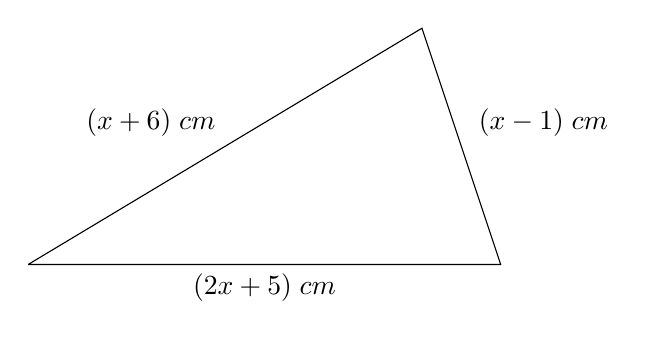
\begin{tikzpicture}
                                \draw (0,0) -- (6,0) node[midway,below] {$(2x+5)\;cm$}
                                            -- (5,3) node[pos=0.6,right, xshift=2mm] {$(x-1)\;cm$}
                                            -- (0,0) node[pos=0.4,left, xshift=-5mm] {$(x+6)\;cm$};
                         \end{tikzpicture}\end{center}
		   
               \begin{envSolution}[height=4cm]
		            $\begin{mArrow}
		               &  \quad                       \\ 
                       &  \quad      						  
	              \end{mArrow}$
               \end{envSolution}			  
	           \begin{shortsolution}$\quad$\end{shortsolution}
\end{enumerate}

\clearpage 
\begin{enumerate}[resume]	
  \item The rectangle below has dimensions as shown.
                         \begin{center}\begin{tikzpicture}
                               % Rectangle with labeled edges
                                 \draw (3,0)  -| (8,3) 
                                    node[pos=0.25,below] {$(2x+3)\;cm $} 
                                    node[pos=0.75,right] {$(2x-3)\;cm $}
                                    -| (3,0);
                         \end{tikzpicture}\end{center}
		\begin{enumerate}[label=(\alph*)]
           \item Find an expression for its perimeter.		   
               \begin{envSolution}[height=4cm]
		            $\begin{mArrow}
		               &  \quad                       \\ 
                       &  \quad      						  
	              \end{mArrow}$
               \end{envSolution}			  
	           \begin{shortsolution}$\quad$\end{shortsolution}
           \item Find an expression for its area.		   
               \begin{envSolution}[height=4cm]
		            $\begin{mArrow}
		               &  \quad                       \\ 
                       &  \quad      						  
	              \end{mArrow}$
               \end{envSolution}			  
	           \begin{shortsolution}$\quad$\end{shortsolution}
		\end{enumerate}
\end{enumerate}

\begin{enumerate}[resume]	
  \item \begin{exercise} A shop sells shirts for $x$ and jackets for $(x + 5)$. The shop sells 6 shirts and 4 jackets for a total of $120$.\\
                         Write down and solve an equation to find the cost of one shirt.
           \begin{envOut}[height=6cm]{bAnswer}
		      $\begin{mArrow}
		            &  \quad                       \\ 
                    &  \quad      						  
	           \end{mArrow}$
           \end{envOut}			  
	       \begin{shortsolution}  
	            $\quad$
           \end{shortsolution}
	  \end{exercise}


  \item \begin{exercise} The cost of a magazine is $\$(x-10)$ and the cost of a book is $\$x$. The total cost of 2 magazines and 5 books is $\$85$.\\
                         Write down and solve an equation in $x$ to find the cost of a magazine.
           \begin{envOut}[height=6cm]{bAnswer}
		      $\begin{mArrow}
		            &  \quad                       \\ 
                    &  \quad      						  
	           \end{mArrow}$
           \end{envOut}			  
	       \begin{shortsolution}  
	            $\quad$
           \end{shortsolution}
	  \end{exercise}
\end{enumerate}	  

\begin{enumerate}[resume]
  \item Write an algebraic expression for each of the following. Let $x$ be the number.
  \begin{subtask}(2)
    \task[] \begin{exercise} Eight is subtraced from the number.
               \begin{envOut}[height=3cm]{bisAnswer}
			       $\begin{mArrow}
			                x - 8	   
	                \end{mArrow}$
               \end{envOut}			  
			  \begin{shortsolution}  
				       $x-8$
			  \end{shortsolution}
		    \end{exercise}

    \task[] \begin{exercise} The number divided by five.
               \begin{envOut}[height=3cm]{bAnswer}
			       $\begin{mArrow}
			                \frac{x}{5}	   
	                \end{mArrow}$
               \end{envOut}			  
			  \begin{shortsolution}  
				       $\frac{x}{5}$
			  \end{shortsolution}
		    \end{exercise}

    \task[] \begin{exercise} Double the number minus ten.
               \begin{envOut}[height=3cm]{bAnswer}
			       $\begin{mArrow}
			                2x-10	   
	                \end{mArrow}$
               \end{envOut}			  
			  \begin{shortsolution}  
				       $2x-10$
			  \end{shortsolution}
		    \end{exercise}
			
    \task[] \begin{exercise} Seven more than half of the number.
               \begin{envOut}[height=3cm]{bAnswer}
			       $\begin{mArrow}
			                \frac{x}{2} +7	   
	                \end{mArrow}$
               \end{envOut}			  
			  \begin{shortsolution}  
				       $\frac{x}{2} +7$
			  \end{shortsolution}
		    \end{exercise}

   \end{subtask} 
\end{enumerate}
\begin{enumerate}[resume]
   \item \begin{exercise} $y$ is 1 more than the square of the sum of $x$ and $m$.
                          Write down a formula for $y$ in terms of $x$ and $m$.
           \begin{envOut}[height=6cm]{bAnswer}
		      $\begin{mArrow}
		            &  \quad                       \\ 
                    &  \quad      						  
	           \end{mArrow}$
           \end{envOut}			  
	       \begin{shortsolution}  
	            $y=(x+m)^2 + 1 $
           \end{shortsolution}
  	    \end{exercise}
\end{enumerate}

\begin{enumerate}[resume]
   \item \begin{exercise} Bus tickets cost $\$5$ for an adult and $\$3$ for a child. There are $a$ adults and $c$ children on a bus. The total number of people on the bus is 30. The total cost of the 30 tickets is $\$128$.\\
Find the number of adults and the number of children on the bus.
           \begin{envOut}[height=6cm]{bAnswer}
		      $\begin{mArrow}
		            &  \quad                       \\ 
                    &  \quad      						  
	           \end{mArrow}$
           \end{envOut}			  
	       \begin{shortsolution}  
	            $\quad $
           \end{shortsolution}
  	    \end{exercise}
\end{enumerate}	  	  